\documentclass{sig-alternate}
\usepackage{url}
\usepackage[flushleft]{threeparttable}
\begin{document}

\title{A Case Study in Preserving a\\High Energy Physics Application}
\author{
Haiyan Meng, Matthias Wolf, Peter Ivie, Anna Woodard, Michael Hildreth, and Douglas Thain\\
\affaddr{Department of Physics and Department of Computer Science and Engineering}\\
\affaddr{University of Notre Dame}\\
\affaddr{\{hmeng|mwolf3|pivie|awoodard|mhildreth|dthain\}@nd.edu}
}
\date{15 January 2014}
\maketitle

\begin{abstract}
\it The reproducibility of scientific results increasingly
depends upon the preservation of computational artifacts.
Although preserving a computation to be used later sounds
easy, it is surprisingly difficult due to the complexity
of existing software and systems.  Implicit dependencies,
networked resources, and shifting compatibility all conspire
to break applications that appear to work well.  To investigate
these issues, we present a case study of a complex high energy
physics application.  We analyze the application and attempt
several methods at extracting its dependencies for the purposes
of preservation. 
We propose one fine-grained dependency management toolkit to preserve the application and demonstrate its correctness in two different environments - one virtual machine from Notre Dame Cloud Platform and one virtual machine from Amazon EC2 Platform. 
We report on the completeness, performance,
and efficiency of each technique, and offer some guidance for
future work in application preservation.
\end{abstract}

% A category with the (minimum) three required fields
%\category{H.4}{Information Systems Applications}{Miscellaneous}
%A category including the fourth, optional field follows...
%\category{D.2.8}{Software Engineering}{Metrics}[complexity measures, performance measures]

%\terms{Theory}

\section{Introduction}

Reproducibility is a cornerstone of the scientific process~\cite{borgman2012data}.
In order to understand, verify, and build upon previous work,
one must be able to first recreate previous results by applying
the same methods. Historically, reproducibility this has been
accomplished through painstaking detailed documentation recorded
in lab notebooks, which are then summarized in peer-reviewed publications.
But as science increasingly depends on computation,
reproducibility must also encompass the environments, data, and software
involved in each result~\cite{zabolitzky2002preserving}. It is widely recognized that informal
descriptions of software and systems -- although common -- are insufficient
for reproducing a computational result accurately.
A more automated and comprehensive approach is required.

The overall reproduction of a computation has three broad components,
each of which suggests somewhat different approaches:

\begin{itemize}
\item The {\bf computing environment}, consisting of the basic hardware and the operating system can be preserved as physical artifacts or as a combination of virtual machine monitor (hardware) and virtual machine image (operating system)~\cite{matthews2009towards}.
\item The {\bf scientific data} to be analyzed has historically received the most attention for curation.  In a large, well-organized project, it may be stored in a  data repository or database management system, with associated documentation and a curation strategy.  In a small effort, it could simply be a handful of files.
\item The {\bf software environment} includes the source code, binaries, scripts, configuration files, and everything else needed to execute the desired code.  As with data, the software could be drawn from a well-managed software repository, or it could be a handful custom scripts that exist in the user's home directory.
\end{itemize}

In a very abstract sense, reproducing a computation is trivial.
Assuming a computation is deterministic, one must simply
preserve all of the inputs to a computation, then re-run
the same code in an equivalent environment, and the same result
will be produced.  For a small custom application on a modest
amount of data, this could be accomplished by capturing the environment,
data, and software within a single virtual machine image,
and then depositing the virtual
it into a curated environment.  The publication could
then simply refer to the identifier of the image, which the
interested reader can obtain and re-use. This approach has
been used to some success with systems like JVM~\cite{barthe2008preservation}.
\footnote{Of course, we are glossing over the problem that hardware
architectures and virtual machines also change, so one must also
preserve the VMM software necessary to run the image.  The VMM itself
depends on a software environment which must also be preserved.
A long-term preservation system might end up running a whole
stack of nested virtual machines in order to provide the desired
environment! }

However, this simple approach is not sufficient for large applications
that are run in complex social environments.

\begin{itemize}
\item There may be {\bf implicit dependencies} on items that are
not apparent to the end user.  For example, they may understand that
they rely on a particular data analysis package, but would have
no reason to know that the package has further dependencies on
other libraries and configuration files.  Or, they may know that
the computation only runs correctly on a particular machine, but
not know this is because it relies on data in a filesystem that
is mounted only on that machine.

\item The {\bf granularity} of the dependencies may not be well understood.
For example, the user may understand that a computation depends upon
a data collection that is 1TB in overall size, but not have detailed
knowledge that it only requires three files totalling 300MB out of that
whole collection

\item There may be dependencies upon {\bf networked resources} that
are inherently external to the system, such as a database, a code
repository~\cite{cms2006cmssw}, or a scalable filesystem~\cite{blomer2011cernvm}.  For such resources, it
must be decided whether the dependency will simply be noted, or if it
must be incorporated whole or in part.

\item Where {\bf common dependencies} are widely used, it may be inefficient or
impossible to store one copy of each dependency for each archived object.
Some form of sharing or de-duplication is necessary in order to keep
the archive to a reasonable size.
\end{itemize}

We do not claim to have solved these problems in any comprehensive
way.  Rather, our aim in this paper is to highlight the scope
of the problems by presenting a case study of one complex application.
The application is presented to us
first in the form of an email that describes in prose how to install
the software and run the analysis.  We perform several successive
refinements to convert it into an executable and preservable object.
Then, we develop two techniques for observing and capturing the
dependencies associated with the system, comparing the cost of capture,
the size of the preserved object, and the flexibility of the resulting
object.  
We propose one fine-grained dependency management toolkit to preserve the application and demonstrate its correctness in two different environments - one virtual machine from Notre Dame Cloud Platform and one virtual machine from Amazon EC2 Platform. 
We describe how each of these techniques may interact with
a future archive of preserved software artifacts, and conclude with
some reflections on the challenges of preservation and advice for future efforts.

\if 0
Section 2: Overview of Application
    CMS/LHC introduction.
    Data sources and reduction of size.
    Code sources and reduction of size.
    Prose observations about the script.
        Uses multiple repos that change over time, with varying level of stability.
        Low selectivity from the larger repos
        Significant initialization time to collect everything.
        Incidental infrastructure tools versus essential objects.
        Some dependencies were surprising.
    Figure: Diagram of app with both code and data sources.
    Table: Show all code and data sources and size within one table.

Section 3: Preservation Strategies
    Figure: Show app in four stages:
        Single email.
        Script with embedded references to dependencies.
        Script with map file that refers to external dependencies.
        Script with map file that refers to preserved dependencies.

    Transform to more suitable format that expresses dependencies.

    Incorporate into archive, saving deps and map file.

    But, how to get the dependencies?

    Three strategies:
        Original - Unmodified application run in original environment.
        Coarse-Grained - Capture deps at large granularity -- whole filesystems and repositories.
        Fine-Grained - Capture deps at a fine granularity -- individual files actually used.

    Coarse-Grained Method (Copy Repositories)
        First, determine dependencies
        Express app as script + map file
        Packaging tool downloads deps, rewrites map file.
        To run packaged application, obtain map, download

    Fine-Trained Toolkit (Parrot)
        Tool to detect dependencies (Parrot)
        Express app as script + map file
        Packaging tool downloads deps, rewrites map file.
        To run package application, run again with Parrot.

Section 4: Evaluation

    Table: Time and size of preserving using each of the two techniques.

    Explain why the techniques show different performance.

    Is one technique more effective than the other?  Why?
\fi

\begin{figure}[t]
\centering
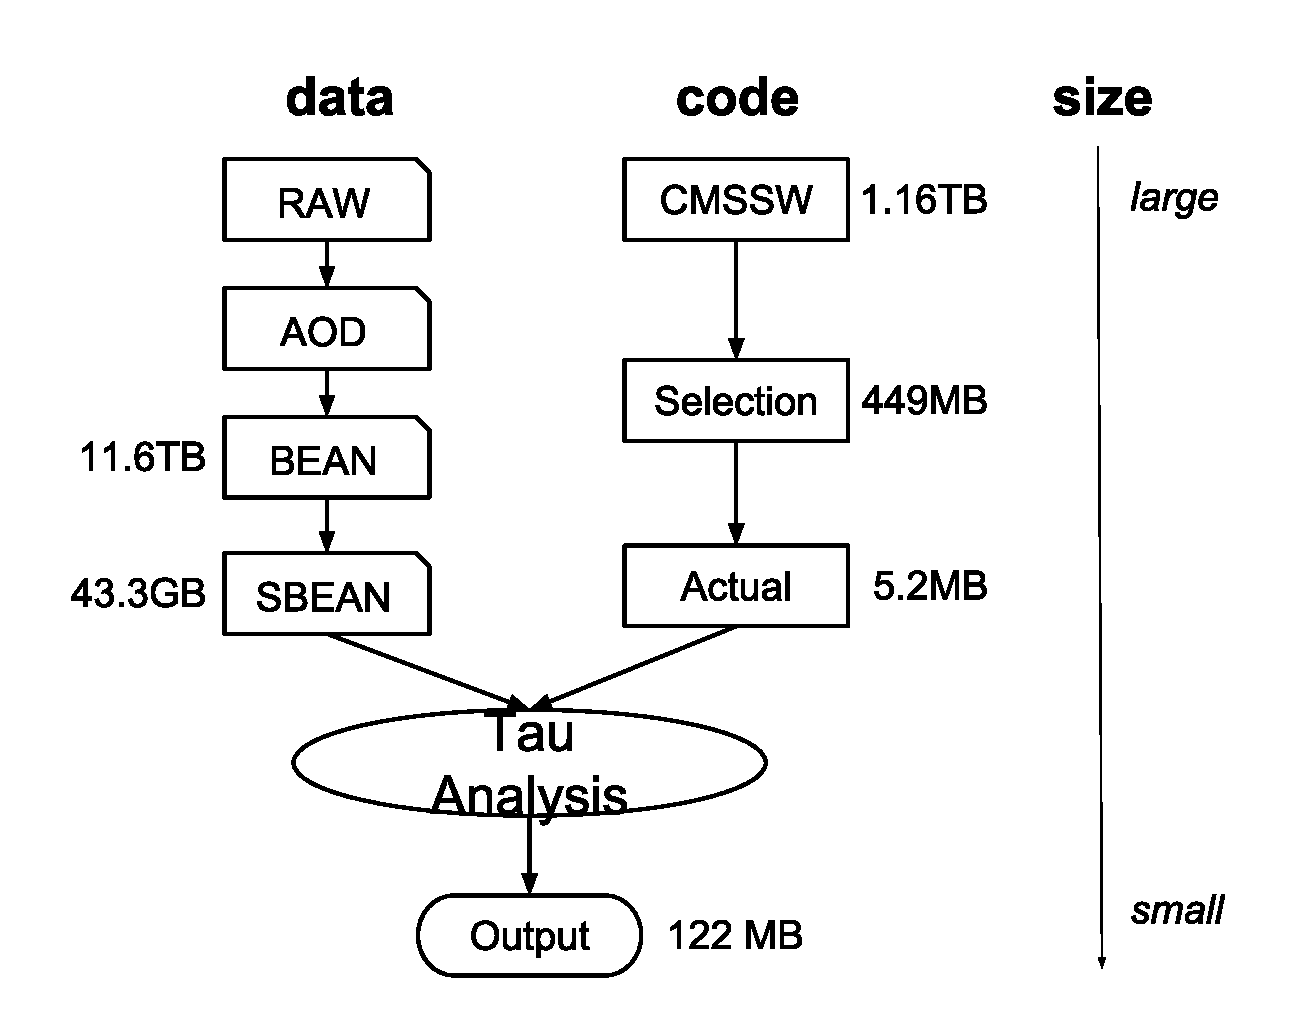
\includegraphics[width=.8\columnwidth]{data-code-size.eps}
\caption{Inputs to Tau Roast}
\label{fig:data-code-size}
\end{figure}

\begin{table}[t]
    \centering
    \small
    \begin{tabular}{|l|l|r|r|r|}
        \hline
        \bf Name & \bf Location & \bf Total & \bf Named & \bf Used \\ 
        \hline
        CMSSW code     & CVS & 88.1GB & 448.3MB & 6.3MB\\ \hline
        Tau source       & Git & 73.7MB & 73.7MB & 6.7MB \\ \hline
        PyYAML binaries    & HTTP & 52MB & 52MB & 0KB \\ \hline
        .h file       & HTTP& 41KB & 41KB & 0KB \\ \hline \hline
        Ntuples data    & HDFS& 11.6TB & 43.3GB & 20GB \\ \hline
        Configuration & CVMFS & 7.4GB & N/A & 103MB \\ \hline
        Linux commands & localFS & 110GB &  N/A & 68.4MB \\ \hline     
        HOME dir& AFS &12GB & N/A & 32MB\\ \hline
        Misc commands & PanFS & 155TB & N/A  & 1.6MB \\ \hline
        Total      &    & 166.8TB            & N/A & 21GB \\ \hline
    \end{tabular}
    \begin{tablenotes}
      \small
      \item The first column illustrates the total size of each data and software source; 
            the second column illustrates the size of the named files from each source;
            the third column illustrates the size of actually used data from each source.
            N/A denotes it is hard to figure out the named size of implicit dependencies directly.        
    \end{tablenotes}
    \caption{Data and Code Used by Tau Roast}
    \label{table:size-original-real}
\end{table}

\section{Overview of Tau Analysis}

Within the ongoing investigation of the Higgs boson at the CMS
detector, part of the LHC at CERN~\cite{collaboration2008cms}, the Higgs production in association
with two top quarks allows to measure the Higgs coupling strength to
top quarks.  As the Higgs boson is to short-lived to be detected
itself, it has to be reconstructed from its decay products.

The application which is the study of this paper is called \emph{TauRoast}
It searches for cases where the the Higgs boson decays to two tau leptons.
The leptons are not observed directly, but by the particle showers
that they generate.  So, the analysis must search for detector
events that show a signature of decay products compatible with both hadronic tau and top decays.  Properties of such events are used to distinguish
the events of interest (Higgs decays) from all other events and
are also used in further statistical analysis.

Figure~\ref{fig:data-code-size} shows that both the code and data
that form \emph{TauRoast} are drawn from large repositories through
multiple steps of reduction.

{\bf Data Sources.}
The CMS collaboration provides analysis end-users with a pre-processed
and reduced data format, AOD~\cite{holtman2001cms}, containing information for events, i.e.,
proton-proton collisions with a signature of interest, in the form of
reconstructed particles.  This format is based on the RAW output of
the CMS detector readout electronics and reconstructed world-wide.
Both real and simulated data are available for examination.

As AOD data are too large to be iteratively processed repetitively in
an physics analysis workflow, it is normally reduced further in
structural complexity and content.  For the analysis under
investigation here, this is a two-step process.  First, the AOD data
are processed at the Notre Dame working group cluster to BEAN events,
containing only trivial data containers packed in vectors.  This step
is time and CPU intensive and its output contains data of 11.6$\,$TB to be
analyzed by the tau analysis.
It is performed by a small custom code framework,
which is built on top of the CMS software stack, CMSSW~\cite{cms2006cmssw},
and uses packages provided by several other special interest groups within CMS.
While the CMSSW framework is installed locally,
the various packages used are checked out from CVS,
and the BEAN framework is stored in git.
This is scheduled to change,
as the CMSSW distribution model switches to a virtual filesystem mounted via FUSE,
and special interest groups move their code to git.
The BEAN format, production code, and
data are shared within the analysis group looking at Higgs production
in association with top quarks, which is formed by groups from a few
American and European universities,
consisting of up to a few dozen contributors.

In the second step, which is the beginning of the actual tau analysis,
the data are reduced to variables relevant to the tau roast procedure, while
only events matching basic quality criteria are kept.  This results in
a dataset of 43.3$\,$GB.  Again, the Notre Dame CMS groups cluster
resources are used to perform this reduction and selection,
running highly customized software,
built on CMSSW and the BEAN framework,
but with output code written and maintained by a few people only.
Again, the code is stored in a git repository.

The final data analysis, investigated below, can be run as a single
process, and contains a stringent event selection to keep only high
quality candidate events for the underlying physical process (using
about 20$\,$MB of space).  Quantities from the selected events can be
both plotted and used in multivariate analysis to determine the level
of expected signal in real data.
This package is written using the CMSSW build framework,
but only utilizes code from ROOT,
a particle physics toolkit underlying CMSSW,
and a few external python dependencies for convenience.
The latter have to be manually fetched and installed,
while the analysis program is built by CMSSW after being checked out of git.

{\bf Code Sources.} Like many scientific codes, the central algorithm
of \emph{TauRoast} is expressed in a relatively small amount of
custom code developed by the primary author.  But, the code cannot
run at all without making use of an enormous collection of software
dependencies.  Some of these dependencies are standard to operating
systems worldwide, some are standardized across the entire high-energy
physics field, some are particular to small collaborative groups,
and a few are very specific to a single researcher.

The largest of these repositories is the CMS Software Distribution (CMSSW),
a carefully-curated selection of software packages which is distributed
in several forms.  Historically, components of CMSSW were obtained by checking components
of the source out of CVS, or by installing a complete binary package on a shared
filesystem within an HPC center.  In recent years, distribution has moved to
an on-demand delivery system known as CVMFS~\cite{blomer2011cernvm}.  The content
of CMSSW is managed very carefully by a centralized team whose main goal
is to ensure that the current version of the software operates correctly
on the operating systems and architectures currently in use.  However,
preservation is not an objective of the group, and so there is
no guarantee that old versions of CMSSW operate in new environments,
or vice versa. 

\section{Observations}

\emph{TauRoast} was provided to us in the form of an
email which described, in prose, how to obtain the source,
build the program, and run it correctly on one specific
machine at our home institution, with no particular guarantee that
it will run anywhere else in the world.
Although this starting point may seem extreme, it is
perfectly natural for collaborators to share configurations
with each other in this form, and to rely on the presence
of a working environment with appropriate dependencies already
installed.  From this starting point, the authors played the
role of curators, whose job it is to prepare the application
for permanent archival.

First, we elaborated the email instructions into an
executable script that obtains the dependencies and then
executes the analysis.  The script declares the necessary
environment variables, downloads and checks out the necessary source code,
builds it appropriately, calls initialization scripts in
the dependent software, and then runs the analysis.
A few rounds of correction with the original author were necessary
to obtain all the dependencies and run the artifact correctly.
(The original email also indicated how to run the application
within a production batch system.  For the purposes of preservation,
we consider the execution infrastructure to be distinct from the application,
and leave it out of consideration for now.)

The process of elaborating the program into a script revealed
several observations about this type of application:

\begin{itemize}

\item {\bf Many Explicit External Dependencies.}  TauRoast depends on a large number of
external dependencies, each with a different access method and data source.
While we knew in advance that it depended upon the large CMSSW distribution,
it was not apparent until elaborating the script that it depended upon
two different Github repositories for the Tau source,
a CVS server at CERN for some configuration information, a public web page
for the PyYAML library, and the public home page of a Notre Dame student
for one missing header file.  (The latter is particularly troubling!)
While, at some level, the authors and users of these software know of these dependencies, they are often missing in
informal communications or forgotten once the dependency is install.
However, once known, they are at least expressed explicitly within the script.

\item {\bf Many Implicit Local Dependencies.} A much harder problem is that the
application assumed the presence of many different components in the local
filesystem view. It would be tempting to capture all of these by simply
storing a virtual machine image containing the local filesystem. However,
the application depended on no less than {\bf six} networked filesystems
available on a particular machine available to the author:
the data to be analyzed was stored on an HDFS~\cite{hadoop} cluster,
some configuration data was stored on a CVMFS~\cite{cvmfs} filesystem,
and a variety of software tools were on an NFS~\cite{howard1988scale},
PanFS~\cite{welch2008scalable} and AFS~\cite{sandberg1985design} systems.
The original authors were not aware of many of these dependencies,
because they simply relied on local administrators to configure the
software and make it available.

\item {\bf Configuration Complexity.}  As a means of controlling the complexity
of dependent software packages, the high energy physics community has developed
a number of tools that perform run-time configuration and consistency checks
of the available software.  {\tt scram} is the software management tool used
by the CMS experiment.  Before running any code, {\tt scram} is used to locate
the appropriate version software,  set environment variables such as the PATH, run any
tool-specific configuration, and do the same for all software on which it depends.
If the correct versions are not available, {\tt scram} halts and emits an error.
While this procedure has great value for consistency, it also introduces a significant cost
because it involves a large number of nested scripts traversing a filesystem,
repeatedly looking up metadata.  In our example, the time to perform this configuration
with a cold cache is about 14 minutes, which is almost as large as the actual analysis
run, which takes 20 minutes.

\begin{figure*}[t]
\centering
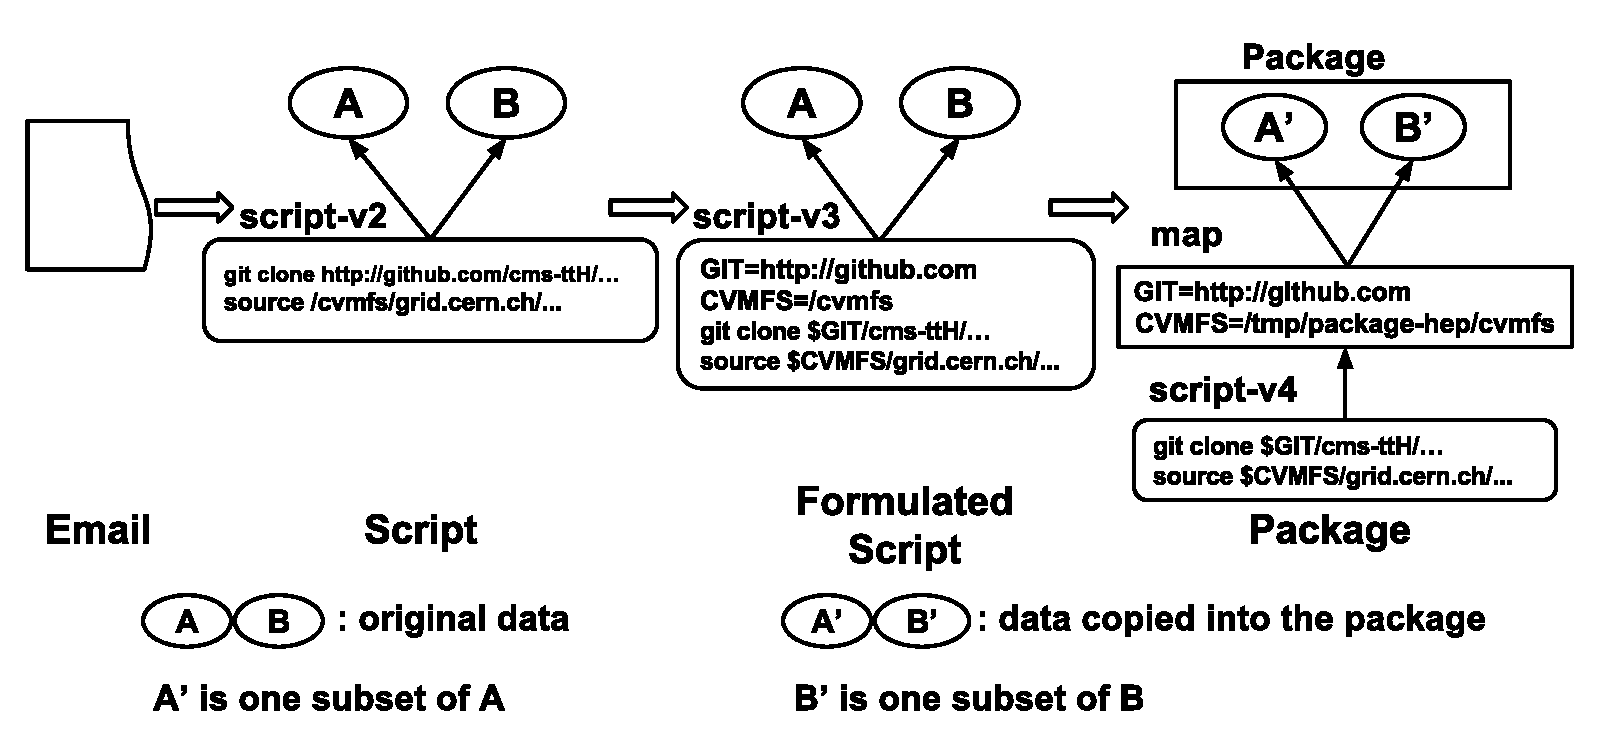
\includegraphics[width=1.6\columnwidth]{version-evolution.eps}
\caption{Version Evolution}
\label{fig:version-evolution}
\end{figure*}

\item {\bf High Selectivity.}  Although the total size of the resources accessed by this
program is very large, the size of the data and software actually used are much smaller.
Often, an entire repository or data source is named within the script, but the program
only needs a handful of items from that source.  For example, the data is stored on an
HDFS filesystem with 24TB of data, but only 43GB of that are the input Ntuples,
and of those only 20GB are actually consumed by the program. The CMSSW repository is 88GB in total
but only 448MB in source are checked out, and the software actually used only
measured 6.3MB.  In a few cases, a source of software is named but never actually accessed.
(For example, our original script includes the Open Science Grid software stack in the PATH, but does not actually use it.)
We suspect that end users are accustomed to missing dependencies and thus get in the habit of adding commonly used software,
whether it is needed or not.

\item {\bf Rapid Changes in Dependencies.}  Over the course of three months
between collecting the initial email, analyzing the program, and writing this
paper, the computing environment was under continuous change.  The CMSSW software
distribution released a new version, the target execution environment was upgraded
to a new operating system, and the experiment deprecated the use of CVS for obtaining
the software.  While the users of this software seem be accustomed to constant change,
any preservation technique will have to be very cautious about relying upon an
external service, even one that may appear to be highly stable.

\end{itemize}

\if 0

\begin{table}
    \centering
    \begin{tabular}{|l|}
        \hline
        {\bf Version 1: Email}\\ \hline
        1. Create a CMS release,\\
            \hspace{9pt} e.g. {\tt cmsrel CMSSW\_5\_3\_11\_patch3} \\
        2. Install the BEAN packages as the instructions: \\
            \hspace{9pt} {\tt \url{https://github.com/cms-ttH/BEAN/blob/...}}\\
        3. Install grid-control: \\ 
            \hspace{9pt} {\tt svn co \url{https://ekptrac.physik.uni-ka/...}} \\
        4. INstall the TauAnalysis package: \\
           \hspace{9pt} {\tt git clone \url{https://github.com/matz-e/...}} \\
           \hspace{9pt} {\tt scram b -j32} \\
        5. Fix grid\_control.cfg and run it. \\
        6. Perform the actual tau roast program. \\ 
        \hline
        {\bf Version 2: Script}\\ \hline
        {\tt setenv CMSSW\_BASE CMSSW\_5\_3\_11\_patch3} \\
        {\tt cmsrel \$HOME/\$CMSSW\_BASE} \\
        {\tt cvs co -r V03-09-23 PhysicsTools/PatUtils} \\
        {\tt git clone \url{https://github.com/cms-ttH/BEAN.git}} \\
        {\tt wget -r \url{http://nd.edu/~abrinke1/...}} \\
        {\tt scram b -j32} \\
        {\tt wget \url{http://pyyaml.org/download/pyyaml/PyYAML...}}\\
        \#the experiment data is from HDFS \\
        {\tt cd \$HOME/\$CMSSW\_BASE/src/PyYAML-3.10}\\
        {\tt cmsenv}\\
        {\tt python setup.py install --user} \\
        {\tt scripts/roaster data/generic\_ttl.yaml} \\ 
        \hline
        {\bf version 3: Formulated Script} \\ \hline
        {\tt setenv CMSSW\_BASE CMSSW\_5\_3\_11\_patch3} \\
        {\tt setenv {\bf GIT} \url{https://github.com}} \\
        {\tt setenv {\bf PYYAML} \url{http://pyyaml.org}} \\
        {\tt setenv {\bf ND} \url{http://nd.edu}} \\
        {\tt cmsrel \$HOME/\$CMSSW\_BASE} \\
        {\tt cvs co -r V03-09-23 PhysicsTools/PatUtils} \\
        {\tt git clone \${\bf GIT}/cms-ttH/BEAN.git} \\
        {\tt wget -r \${\bf ND}\url{/~abrinke1/ElectronEffectiveArea.h}} \\
        {\tt scram b -j32} \\
        {\tt wget \${\bf PYYAML}/download/pyyaml/PyYAML...}\\
        \#the experiment data is from HDFS \\
        {\tt cd \$HOME/\$CMSSW\_BASE/src/PyYAML-3.10}\\
        {\tt cmsenv}\\
        {\tt python setup.py install --user} \\
        {\tt scripts/roaster data/generic\_ttl.yaml} \\ 
        \hline
       {\bf Version 4: Fine-Grained Toolkit - Package}\\ \hline
        {\tt setenv CMSSW\_BASE CMSSW\_5\_3\_11\_patch3} \\
        {\tt setenv {\bf GIT} \url{https://github.com}} \\
        {\tt setenv {\bf PYYAML} \url{http://pyyaml.org}} \\
        {\tt setenv {\bf ND} \url{http://nd.edu}} \\
        {\tt cmsrel \$HOME/\$CMSSW\_BASE} \\
        {\tt cvs co -r V03-09-23 PhysicsTools/PatUtils} \\
        {\tt git clone \${\bf GIT}/cms-ttH/BEAN.git} \\
        {\tt wget -r \${\bf ND}\url{/~abrinke1/ElectronEffectiveArea.h}} \\
        {\tt scram b -j32} \\
        {\tt wget \${\bf PYYAML}/download/pyyaml/PyYAML...}\\
        \#the experiment data is from HDFS \\
        {\tt cd \$HOME/\$CMSSW\_BASE/src/PyYAML-3.10}\\
        {\tt cmsenv}\\
        {\tt python setup.py install --user} \\
        {\tt scripts/roaster data/generic\_ttl.yaml} \\ 
        \hline
    \end{tabular}
    \caption{Scripts of each Solution}
    \label{table:scripts}
\end{table}

\fi

\section{Evolving the Artifact}

It is clear that the artifact, as provided, is not in a suitable form
for preservation.  While it might be technically possible to automatically
capture the entire virtual machine and all of the connected filesystems,
doing so would be wasteful and prohibitively expensive.  Further, if multiple
similar applications are preserved, we would miss the opportunity to identify
common dependencies and store them once for multiple artifacts.

Figure~\ref{fig:version-evolution} shows how we have evolved this artifact
through several stages which make it more suitable for preservation.
In each step of evolution, we make the dependencies of the artifact
more explicit and available for analysis and automated processing.
As noted in the previous section, the original author provided us with
prose instructions by email which we translated into an
executable script.  The executable script has embedded in it
a number of external identifiers such as URLs pointing to repositories
and paths to networked filesystems.  As a general programming practice,
embedding such constants into the middle of a program is unwise, and so
we extract all of those identifiers and place them at the beginning
of the script in the form of variable substitutions.  This makes
it readily apparent to the reader what the dependencies are.

Form 4 goes a step further and takes all of the dependencies \emph{out}
of the script itself and places them in a \emph{dependency map}.
The dependency map lists all of the external dependencies of the application, indicating
the type, how they are accessed, and where they are currently located.
The resulting script then simply refers to abstract file locations such
as \verb!$CMSSW!, while the map file indicates where they are located.
If properly constructed, the script should not refer to any external
resource unless it is indicated in the dependency map.

By extracting the dependencies into the external dependency map,
we introduce great freedom for the curator to move, transform, and otherwise
manipulate the dependencies of the artifact without damaging the artifact itself.
For example, it is straightforward for an automated tool to examine
all of the dependencies in the map, download those that are missing,
and then modify the map to point to the local copies of the dependencies.
(Or, in the case of a dependency upon a reliable external archive,
the map file could continue to point to the original source.)

\section{Fine Grained Dependency Management}

The difficulty of data access authority acquisition enforces us to find out one
solution, in which the reproduction of the original analysis can be done
without any external dependency. One independent and self-contained
package containing all the data and software dependencies is necessary. 
Two questions must be answered for this aim. 

{\bf First, who should be responsible to generate the package?}
Someone may suggest that it should be the responsibility of the original author
to generate the required package. However, letting the original author provide
the package is unrealistic. 
Figuring out the underlying dependencies of
each software is complex and time-consuming and even impossible for the
original author. In this experiment, the machine used for the experiment is one
public machine of physics department, and the original author is one common user without
root authority. The underlying OS and supporting softwares are installed and
maintained by the IT department of the university. On the other hand, the
architecture design of the required package including all the data and software
dependencies is not under the research field of physicists.
Therefore, one packaging utility is necessary to help the original author to generate the package.

{\bf Second, how to figure out the implicit dependencies?}
With the help of the formulated script, we can easily figure out the explicit dependencies.
The requirements of the underlying OS and hardware
architecture can be easily found with system tools such as {\tt uname} or
{\tt lsb\_release}.
However, how to figure out the implicit dependencies needs more concerns, because
directly preserving the whole OS together with the data
stored on the disk of the original machine or the data from other filesystems
mounted as local filesystems, such as HDFS and PanFS, is not feasible. One
efficient mechanism which can figure out the really used parts of all these
filesystems is necessary. 
To do this, the file access details of the application should be tracked and utilized.

\begin{figure}
\centering
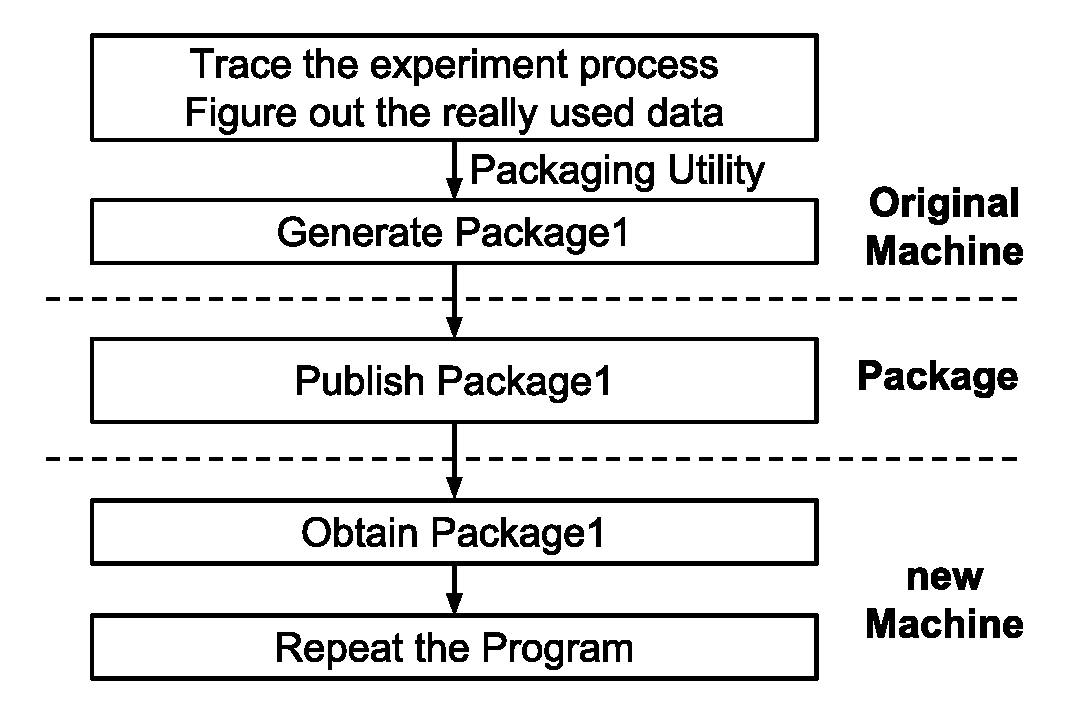
\includegraphics[width=.8\columnwidth]{solution3.eps}
\caption{Relationship of Roles}
\label{fig:solution3}
\end{figure}

The relationship of different roles involved in the experiment preservation and
reproduction is shown in Figure~\ref{fig:solution3}.  The original author uses the packaging utility to generate the package for one application.
Then the package, together with
its map file and description file will be published. When
another researcher wants to repeat the experiment, one copy of the package will be downloaded into the new machine and the application can be repeated.

When we try to repeat one application on one new machine, one map file is necessary for the relocation of the data access targets, as
show in Figure~\ref{fig:version-evolution}. 
The map file clearly defines the real location of each dependency in the format of dependency variables - the real location of dependency variable {\tt GIT} is \path{http://github.com} and the real location of dependency variable {\tt CVMFS}
is {\tt /tmp/package-hep/cvmfs}.
The script only refers to the dependency variables defined in the map file.
This design decouples the experiment script and the actual data access targets, which minimizes the impact of the evolution of different data dependencies
and ensures the transparent access.
The modification of the package only introduces the minimal changes of the map file on the client side.

\section{One Fine Grained Dependency Management Toolkit Based on Parrot}

\begin{figure*}
\centering
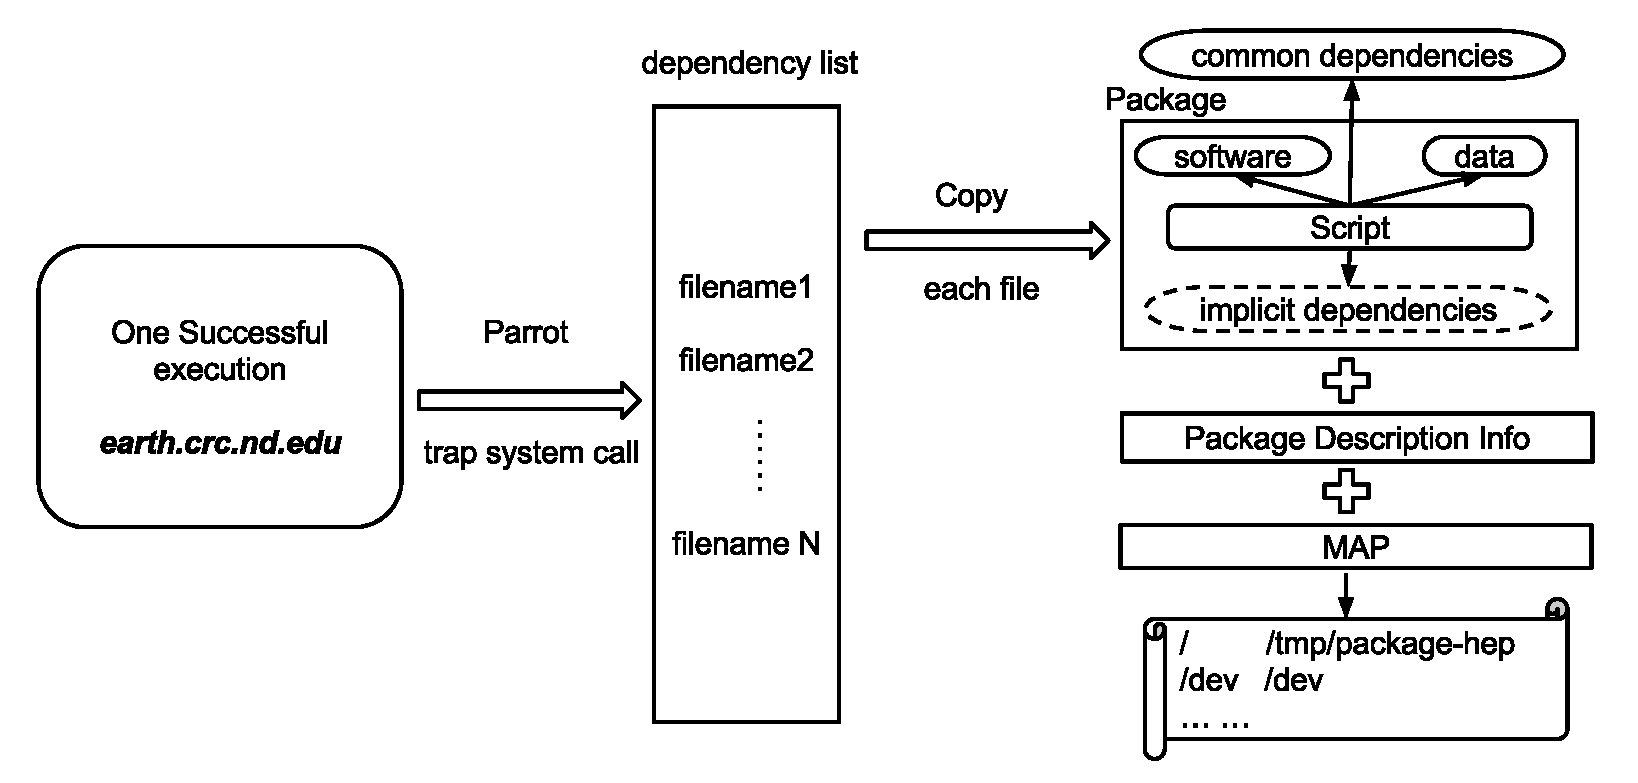
\includegraphics[width=1.6\columnwidth]{workflow-parrot.eps}
\caption{Workflow of The Fine-Grained Dependency Management Toolkit Based on Parrot}
\label{fig:workflow-parrot}
\end{figure*}

With the help of one
virtual filesystem access tool, Parrot~\cite{thain2005parrot}, we trap all system calls of one
program through ptrace debugging interface, and collect all the names of accessed files. 
Then one self-contained package containing all the accessed files is generated to help others repeat the experiment.

Parrot is a virtual filesystem access tool which attaching existing programs to
a variety of remote {\tt I/O} systems including 
HTTP, FTP, GridFTP, iRODS, HDFS, XRootD, GROW, and Chirp. It traps all system calls of one program through ptrace
debugging interface, and replaces them with remote {\tt I/O} operations as desired.

Figure~\ref{fig:workflow-parrot} illustrates the workflow of the fine-grained dependency management toolkit based on Parrot.
The starting point of this toolkit is one successful execution of the application on the native machine.
First, re-execute the actual
data analysis script under Parrot and get the name list of all the files actually
accessed during the data analysis process. Then,
according to the filename list, one package containing all the necessary data
and software for one analysis program is generated. When another
scholar wants to repeat the program, he only needs to obtain the package and
execute the actual analysis program inside the package. 

The filename list contains the names of 132,047 accessed file, together with the access type of each file, such as
open, stat, read and write. 
We noticed that some files appeared multiple times in the filename list. 
De-duplication and sorting techniques are used to deal with the original filename list, generating one smaller list containing 67,168 items.
The total size of each involved directory and file is 900.3GB.

The toolkit iterates each item of the filename list, determines the process
mode and replication degree according to the file type (common files,
directories, symbolic links) and the system call type, generates one package
containing all the necessary file dependencies, and returns the description
information of the package, as shown in Table~\ref{table:package-info}.  To
ensure the successful reproduction, the filesystem structure of the original
execution environment should be preserved as completely as possible. However,
attempting to copy the whole content of one directory or one file is
space-consuming and time-consuming, because the original program may 
only need to know how many items one directory contains and not need the content of the sub-directories or the sub-files.
Our solution is to
determine the replication degree of one directory or one file according to the
system call type. 
If one file is accessed through system calls like {\tt open}, {\tt read} and {\tt write}, the whole content of the file will be copied into the package.
However, if the application only needs to check the existence of one file through {\tt stat} system call, we only create an empty file in the package.
As for a directory item, the sub-items under it will be copied into the package if their contents are necessary. Otherwise, we only create empty sub-items in the package to maintain the directory structure.
The step also runs under Parrot to access data from
different file systems.

\begin{table}
    \centering
    \begin{tabular}{|l|}
    \hline
     the total size of package: 21GB \\ 
    the total number of files: 15905\\ 
    the total number of directory: 1549\\ 
    the total number of symbolic link: 4614 \\ \hline 
    \end{tabular}
    \caption{Package Information}
    \label{table:package-info}
\end{table}

The package, the Parrot executable program, together with the environment description information of the application, such as hardware platform, OS version and kernel version, will be published.

When another researcher wants to repeat the analysis program,
one map file, which maintains the relationship between the file access path referred in the program of the application and the actual file location 
, will be generated, as shown in Table~\ref{table:map-file}.
The path of the package is {\tt /tmp/package-hep}, so the actual location of one file with the original path {\tt path1} will be {\tt /tmp/package-hep/path1}.
However, 
it is impossible to copy the files under certain directories, such as  {\tt /dev}, which contains all the device files.
Each device file is either a block file or a character file. 
The new machine may not share the same device configuration with the original machine, so copying block files into the package is meaningless.
Copying character files such as /dev/tty and /dev/urandom is also meaningless because of their dynamic nature.
It is meaningless to copy the file under the directory {\tt /proc}, 
because OS may allocate different process IDs for multiple executions of one application.
As for these special file paths, letting
the program directly utilize the files on the new machine, where the new user
repeats the program, is a better choice. 
The item {\tt /dev /dev} of Table~\ref{table:map-file}
illustrates this semantics.
With the help of the map file and the package, the application can be repeated on one new machine. 

\begin{table}
    \centering
    \begin{tabular}{|l|l|}
    \hline
    \bf Path used in Program & \bf Actual Location \\ \hline
    {\tt /} & {\tt /tmp/package-hep} \\ \hline
    {\tt /tmp/package-hep} & {\tt /tmp/package-hep} \\ \hline
    {\tt /dev} & {\tt /dev} \\ \hline
    {\tt ...} & {\tt ...}\\ \hline
    \end{tabular}
    \caption{Structure of Map File}
    \label{table:map-file}
\end{table}

\section{Evaluation}
We evaluated the correctness and overhead of the packaging utility of Solution 4.
To do it, the experiment was repeated using Solution 2 and 4 on the original machine.
Then, two different virtual machines (VM) - one VM from Notre Dame Cloud Platform based on KVM and one VM from Amazon EC2 Platform based on Xen, were employed to further verify the correctness of Solution 4.

We first repeated the example from scratch using Solution 2 on the original machine and counted the time consumption and data size. 
Then based on the successful execution of Solution 2, Solution 4 is evaluated - one package containing necessary dependencies is generated, and then the time consumption and data size is analyzed. 

To measure time consumption, we counted the time used to obtain remote software dependencies, build environment, and analyze the dataset respectively. Solution 4 also counted the time used to obtain the filename list and generate the package. To measure data size, we can easily figure out the size of each data and code source easily inside the package under Solution 4.
Solution 2 does not support mining of implicit dependencies. As for remote sources, we can figure out the named size through the analysis script. However, it is hard to figure out the named size of each local source. 
Instead, we only knew that total size of each file system is very large.

Table~\ref{table:time-2nd3rd} shows the execution time comparison between
Solution 2 and 4.
Solution 4 is faster than Solution 2, because all the software copied into the package has been compiled and the Software Acquisition stage is not necessary.
and all the environment building only takes 4 seconds.
We were surprised that Solution 4 even reduces the actual analysis time. 
The reason for this is that data is obtained through accessing HDFS in Solution 2, but is copied into the package in Solution 4. This localization of experimental data speeds up the data analysis process, resulting the actual analysis time reducing from 20 minutes to 13 minutes.

\begin{table}
    \centering
    \begin{tabular}{|l|r|r|}
    \hline
    \bf Task & \bf Solution 2& \bf Solution 4\\ 
    \bf Category & \bf Time & \bf Time \\ \hline
    Obtain filename list & N/A & 28min 28s \\ \hline
    Generate package & N/A & 85min 51s \\ \hline
    Software Acquisition & 8min 11s & N/A \\ \hline
    Environment Build & 5min 49s  & 4s \\ \hline
    Actual Analysis & 20min 31s & 13min 04s \\ \hline
    \end{tabular}
    \caption{Execution Time Comparison between Solution 2 and 4}
    \label{table:time-2nd3rd}
\end{table}    

Table~\ref{table:time-2nd3rd} also illustrates the time used to
obtain the filename list and generate the package. 
The time used for these two steps is longer than the execution time,
because each filename of the list, together with its system call type, needs to be checked, and the structure of each directory item must be maintained.
However, 
this is only done once.
Once the package is
generated, many users can directly obtain the package and repeat the experiment
separately. 

Table~\ref{table:size-original-real} illustrates the total size, named size in the example and actually used size of each remote source (the first 4 items) and local source (the remaining 5 items).
The third column corresponds to the data size of Solution 4 and can be easily figured out, because all the necessary data has been copied into the package.
Solution 2 does not support measuring implicit dependencies. As for remote sources, we can figure out the named size through the analysis script. However, it is hard to figure out the named size of each local source. 
Instead, we only knew that total size of each file system is very large.

To further verify the correctness of Solution 4 on other machines, two different machines are employed -
one virtual
machine~\cite{goldberg1974survey} from Notre Dame Cloud Platform based on KVM sharing the same kernel version with the original machine,
and one virtual machine from amazon EC2~\cite{amazon2010amazon} based on Xen.

Table~\ref{table:config-vm} illustrates the configuration of 
each machine and the execution time of the experiment on each machine.
All the machines adopt x86\_64 hardware platform and Linux OS.
Both of the two VMs repeated the experiment with the help of the package generated on the original machine successfully.
The execution time on one machine greatly depends on its hardware configuration.

\begin{table}
    \centering
    \begin{tabular}{|l|r|r|r|r|}
    \hline
    \bf Machine & \bf Distro & \bf CPU & \bf Mem & \bf Execution\\ 
    \bf Type   &\bf Version&\bf Cores & (\bf GB) & \bf Time\\ \hline
    Native &  Red Hat  & 64 & 125 & 13min 04s\\  
    Machine& 5.10 &&&\\ \hline
    KVM & CentOS & 4 & 2 & 21min 38s\\
    (Notre Dame)&5.10 &&&\\ \hline
    Xen & Red Hat & 16 & 60.5 & 13min 30s\\ 
    (EC2) &5.9 &&&\\ \hline
    \end{tabular}
    \caption{Evaluation of Different Machines}
    \label{table:config-vm}
\end{table}

Regardless, we demonstrate that the application runs correctly in a completely different environment.
%*****hmeng-doubt:Another reason for the packaging utility is that not all the data and software generated by the second version script is used during the the actual data analysis. The packaging utility can help us find out the optimal subset of data and software involved in one actual data analysis. 
%*****hmeng-doubt: this point is not the motivation. but one achievement comes together. out of imagination.

\begin{figure}
\centering
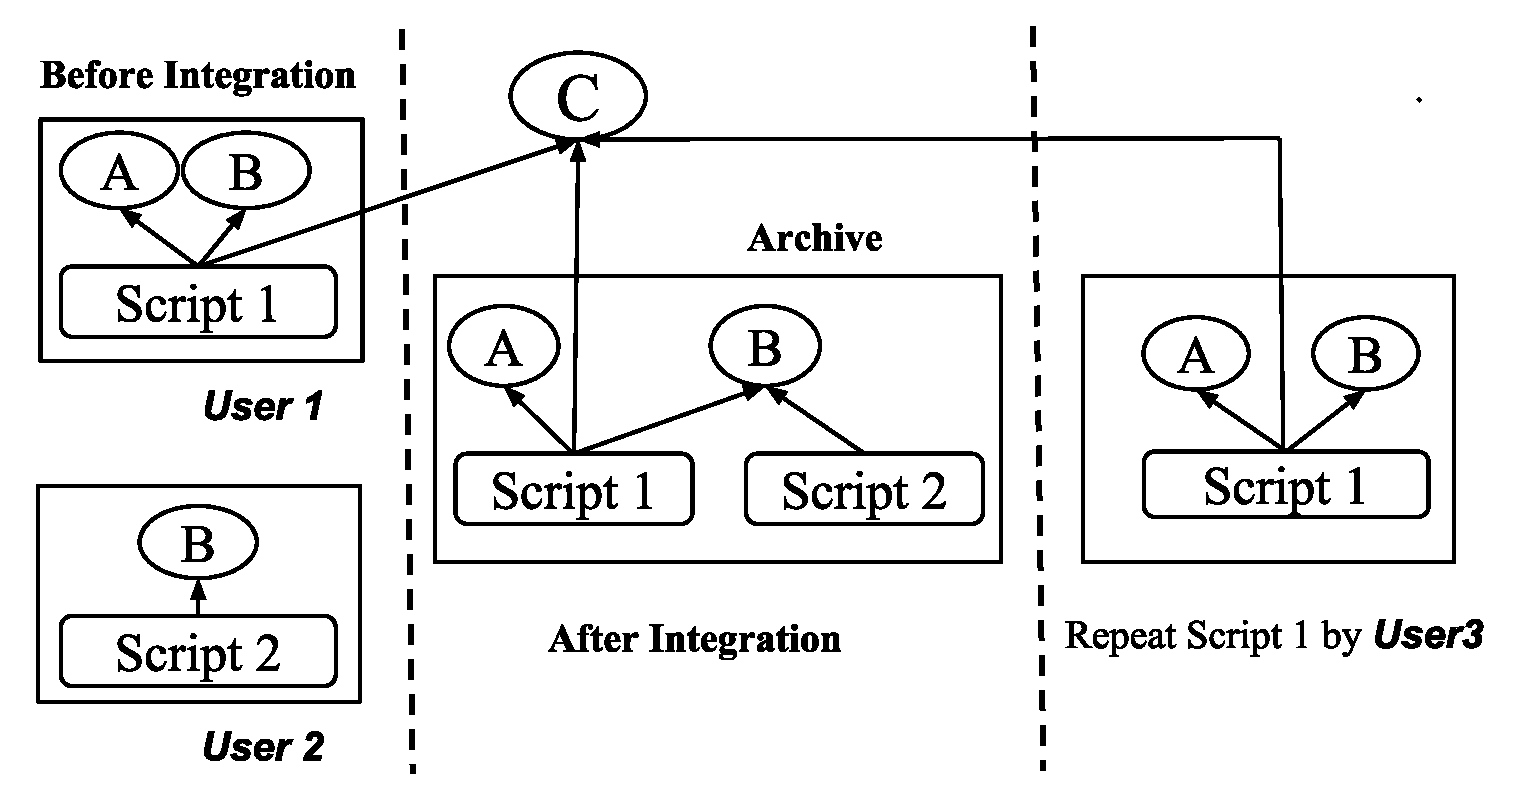
\includegraphics[width=1\columnwidth]{preservation-integration.eps}
\caption{Preserving Multiple Artifacts}
\label{fig:Preservation integration}
\end{figure}

\section{Open Problems}

Figure~\ref{fig:Preservation integration} shows the rough information
architecture of the archive that we imagine for complex
scientific software like TauRoast.
Each artifact to be preserved is a package that consists of a top-level
script to invoke the software, a dependency map, and the dependencies
themselves, which may be external to the original program.  The artifacts
are then ingested into the archive, where shared dependencies are stored
only once.  In cases where an artifact has a dependency on a trusted
(or very large) remote archive, the dependency may simply be tracked
instead of ingested. A researcher that wishes to reproduce a given
result need only refer to the unique identifier of the artifact, and will
be able to automatically extract all of the dependent components of
that artifact.

For example, in Figure~\ref{fig:Preservation integration} Script 1 depends on items A, B, and C.  Items A and B are ingested into the archive, where B is shared with Script 2.  Item C is stored in another trustworthy repository and is tracked rather than ingested.  When Script 1 is exported from the repository, items A and B are exported along with it, while C can be copied or remain remote, according to the end user's choice.

As simple as that picture appears, there are a number of problems that must be solved to get there:

{\bf Measure the Mess or Force Cleanliness?}  Two radically different approaches to dependency tracking are possible.  The first is to allow end users complete freedom to construct their environment as desired, then \emph{measure} what items were actually used.  As we have shown, this is possible, but has significant overheads and does not fully preserve the structure or intent of the end user.   The second approach is to \emph{force} users to work in a clean environment in which no resource can be used until a proper dependency has been declared.  This ensures that all dependencies are known in advance (and made explicit to the end user) but places a variety of restrictions on the user's daily work, and may prevent creative approaches that do not fit within the curator's view of how programs should be structured.  Whether end users will accept the inconvenience of forced cleanliness for the benefits of reproducibility can only be discovered through experiment.

{\bf Granularity of Dependencies.}  Dependencies could be handled
at many different levels of granularity.  In this work, we have shown
how they can be handled at the level of entire repositories or individual files.
Other possible choices might include intermediate-sized software packages
(like RPM) or in the case of experimental data, even portions of individual large files.  Clearly, a larger granularity will result in fewer packages,
simpler dependency maps, and more wasted space; smaller granularity results
in complex dependency maps and less wasted space.  A hybrid solution may
be able to combine both by storing large granularity dependencies, but
retain the ability to select sub-items out of objects when efficiency demands it.

{\bf Scope of Reuse.}  We have presented the data preservation
problem as primarily one of accurate reproduction: if a result depends
on running program X, we must be able to run exactly X again.  However,
the goal of scientific reproducibility is rarely limited to running
\emph{precisely} what a predecessor did. Often, the objective is to
change a parameter or a data input in order to see how the result is affected.
To that end, the preservation system must capture enough of the surrounding
material to permit modifications to succeed.  From this perspective,
a larger granularity of preservation is desirable.  A better understanding of
how end users will consume preserved software will help to shape how
software is preserved in the first place.

{\bf Dependency Detection.}  If we allow users to work in uncontrolled
environments, then we must have better methods for understanding the dependencies  of existing programs.  At first, we relied on an expert reader to examine
the user's script and extract the repository dependencies.  This is clearly
not a scalable approach.  We then demonstrated an automated method of observing
what individual files are accessed by a program. However, this does
not cover all types of dependencies, particularly those that are networked.
More sophisticated observation techniques could infer higher-level information,
such as the RPM package names of the files accessed, the URLs of remote
repositories named throughout the program, or even the addresses and names of networked dependencies like databases and filesystems.

{\bf Source, Binary, or Both?}  A science archive might choose to retain
the source code of an artifact or the binary code that can actually run in a given environment.
While conventional wisdom suggests that access to source code is critical for the long term
survival and evolution of a piece of software, it also requires the maintenance of an enormous
amount of supporting software in the form of compilers, linkers, and supporting libraries for
the target platform.  Rebuilding all of these for every invocation of an artifact is
likely to have excessive cost.  We suggest that a realistic repository will have to
maintain \emph{both}: the source describes the ultimate meaning of the code, but
the binary is an important performance cache, a backup if the compiler toolchain should
fail to be preserved, and a checksum to ensure that a source artifact was rebuilt correctly.

\section{Related Work }

Generally, there are three approaches to preserve software environment:
hardware preservation, migration and emulation.  Hardware
preservation preserves the original software and its original operating
environment. 
Software migration technique~\cite{cifuentes1996binary,mancl2001refactoring} was used to facilitate running software on new machines.
However, migration often involves the re-compiling and re-configuring
the source code to accustom a new hardware platform and software environment.
Emulation recreates the original software and hardware environment by
programming future platforms and OSs. One common solution to implement this is
virtual machine. According to the usage and emulation degree of the real
machine, virtual machine can be divided into system virtual machine and process
virtual machine. 
The working principle, design principle and
performance evaluation of system virtual machine were illustrated in~\cite{goldberg1974survey, smith2005architecture}. 
The
functionality of system VM to support different guest operating systems was illustrated in~\cite{barham2003xen,kivity2007kvm,rosenblum1999vmware}.
F. Esquembre~\cite{esquembre2004easy} illustrated how JVM, one process virtual machine, can expedite the creation of
scientific simulations in Java. 
The pros and cons of these three approaches were discussed in~\cite{matthews2009towards,phelps2005no,hong2010software}.

The preservation of computing environment and software environment was treated as one entirety in~\cite{matthews2009towards,phelps2005no,hong2010software}. However, frequently changing experiment software makes the maintenance of the preserved experimental environment very complex. 
CernVM~\cite{buncic2010cernvm} treated them as two different categories. The preservation of computing environment is implemented with CernVM, and the preservation of software environment is based on a CernVM filesystem(CVMFS) specifically designed for efficient software distribution.

The importance of preserving software in source code format was emphasized in~\cite{zabolitzky2002preserving,castagne2013consider}. 
However, CVMFS~\cite{buncic2010cernvm} published pre-built and configured experiment software releases to avoid repeating the time-consuming software building procedure. 

Attempts from different perspectives to facilitate the reproduction of scientific experiments utilizing preserved software library has been made. 
The software distribution mechanism over network was discussed in~\cite{compostella2010cdf, blomer2011cernvm}.
J. R. Rice et al.~\cite{rice1996scientific} made the reproduction process easier through the integration of user interface, scientific software libraries, knowledge base into problem-solving environment.
S. R. Kohn et al.~\cite{kohn2001divorcing} tried to enable the creation and distribution of language-independent software library by addressing language interoperability.
a scalable, distributed and dynamic workflow system for digitization processes was proposed in~\cite{schoneberg2013scalable}.
A distributed archival network was designed in~\cite{subotic2013distributed} to facilitate process-oriented automatic long-term digital preservation.
M. Agosti et al.~\cite{agosti2012envisage} aimed to help non-domain users to utilize the digital archive system developed for domain experts.

Current mechanisms of preserving scientific experiments assume that all the data and software mentioned in the experiments are necessary for the reproduction of the experiments. However, this is not always right. In some cases, the original author may leave additional code referring to irrelative data and software in the experiment programs. One mechanism, which can figure out the absolutely relevant data and software of one experiment, is important for both the preservation and reproduction of scientific experiments.

B. Matthews et al.~\cite{matthews2008significant} introduced one conceptual framework for software preservation from several case studies of software preservation.
One tool to capture software preservation properties within a software environment was designed in~\cite{matthews2010framework} through a series of case studies conducted to evaluate the software preservation framework.
L. R. Johnston et al.~\cite{johnston2014workflow} proposed one overall data curation workflow for 3-5 case studies of preserving research data.
Two case studies~\cite{borgman2012data} were conducted to figure out the properties of data to be reused in the future, including type, purpose, new users.
To figure out how to preserve HEP applications, this paper studies one case of preserving one representative HEP application.

\section{Postscript}
By the way, at the beginning of our case study, we generated one package for the
example based on Solution 4. Several months later, the original machine met
some problems and the access model of CMSSW was also modified. In this case, if
you want to repeat the example on the original machine, different 
configurations, including CMSSW\_ARCH, environment variables and CVS access
authority need to be modified. However, with the generated package and its map file, we can repeat the experiment directly on the same machine without any modification.

\bibliographystyle{abbrv}
\bibliography{cclpapers,this}

\end{document}
